\section{Data Import}
\label{sec:dataimport}
We realize that the task of importing data into a database as complex as {\germinate} may be overwhelming at first. This is why we try to come up with tools that make this process simpler and faster. In this section, we will highlight some of the possible ways you might want to use to import your data into the {\germinate} database.

\subsection{Germinate Daim}
There are several ways to import data into {\germinate}. Some people may prefer to write their own scripts to import the data whereas others may prefer database management tools like \textit{Navicat} \cite{Navicat} or \textit{MySQL Workbench} \cite{MySQLWorkbench}.

However, we believe that we can make the import process even easier and so we developed a Java based desktop application to aid in the upload of experimental datasets into {\germinate}. The aim of this tool is to simplify the process of entering data into the system. \textit{Germinate Daim} allows permitted MySQL system users to upload data in text file format into a specified {\germinate} installation. We have also included tools to revert the most recent change should any problems arise in the data upload process.\\
\\
 Germinate Daim can be downloaded here:

\begin{center}
    \url{http://ics.hutton.ac.uk/germinate-daim/}
\end{center}

\begin{figure}
    \centering
    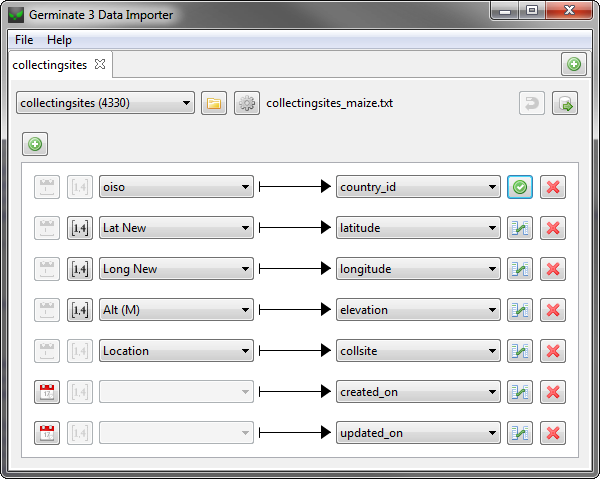
\includegraphics[scale=0.6]{img/import/g3di-mapping.png}
    \caption{Germinate Daim - Column mapping}
    \label{fig:g3di-mapping}
\end{figure}

\noindent Figure \ref{fig:g3di-mapping} shows the main GUI of G3DI with an example mapping. The current tab is used to import data from a text file with the name \texttt{collectingsites\textunderscore maize.txt} into the database table \texttt{collectingsites}. Each row represents a mapping between column of the input file and column of the database. Germinate Daim is aware of the data types of the database columns and provides functionality to accommodate dates, number formats and foreign keys. The first row of the mapping maps \texttt{oiso} (which is a 3-digit country code) to \texttt{country\textunderscore id}. Germinate Daim knows that \texttt{country\textunderscore id} is a foreign key column and requests the user to define a lookup table and column. This lookup is used to find the foreign id based on the value in the \texttt{oiso} column.

As an example, let's assume the lookup table is \texttt{countries} and the lookup column is \texttt{country\textunderscore code3} and the value in the column \texttt{oiso} is "GBR". Germinate Daim will then query the database and determine the id of the country with the 3-digit code "GBR" (which is the United Kingdom) and use this id instead of the actual value.

In addition you can define a number format (or to be exact, a locale) for decimal columns. This format is used to parse your input data before inserting it into the database.

Finally, you can define date formats for columns that represent dates. As an example, let's say your input data is in the form \texttt{dd/MM/yyyy} (2-digit day, 2-digit month, 4-digit year). Germinate Daim will then parse your dates before inserting them into the database. This is necessary, since the database uses its own date format which may differ from the format you used for your data.\\
\\
After you imported your data, you might realize that your mapping was incorrect. Germinate Daim can undo the most recent import step with one click of a button, to allow you to do your work without worrying that you might mess up the database. If you want to be on the safe side, you can still take a backup of the whole database with your favourite database management tool.

\subsection{{\germinate} Data Templates}
Over the years we have learned that people really like Microsoft Excel and that most of the data is stored in Excel spreadsheet before it goes into {\germinate}. To make the best of this fact, we decided to design Excel data templates that specify exactly how your data needs to be formatted for {\germinate} to import it automatically.

The "datatemplates" folder in the {\germinate} source code contains templates for genotypic data, genetic maps, germplasm passport data, pedigree information and trials data. Each of the files contains detailed information about how we require the data to be formatted.

\todo{Explain command line tools}

\subsection{Data Standards}
\todo{fill}
\subsubsection{Dublin Core}
{\germinate} supports the Dublin Core Metadata Element Set \cite{DublinCore} of 15 core terms. These can be associated with a dataset by using the json column \texttt{datasets.dublin\textunderscore core}. Each element of the set is optional, so can either be set to \texttt{null} or left out of it is not required. All elements are arrays, so that multiple values are possible for each key. An example can be seen below:

\begin{lstlisting}[style=JavaScript]
{
	"title": ["An amateur's guide to roasting Unicorns."],
	"subject": ["Unicorns", "Roasting", "Guide"],
	"description": ["Illustrated guide to roasting unicorns. Includes detailed information about the habitat of unicorns and the best way to roast them."],
	"type": ["Text", "Images"],
	"source": ["Deepest depths of a weird mind"],
	"relation": null,
	"coverage": ["2000-2017"],
	"creator": ["Raubach, Sebastian"],
	"publisher": ["The James Hutton Institute"],
	"contributor": null,
	"rights": ["Access limited to everyone except the creator."],
	"date": ["2017-09-28"],
	"format": ["text/plain"],
	"identifier": ["1223-45567-8998"],
	"language": ["English", "German"]
}
\end{lstlisting}